\documentclass[10pt,a4paper]{article}
\usepackage[utf8]{inputenc}
\usepackage{amsmath}
\usepackage{amsfonts}
\usepackage{amssymb}
\usepackage{graphicx}
\author{Jos\'e Miguel Leyva De la Cruz}
\title{Segundo Proyecto de Programaci\'on Matcom Primer A\~no}
\date{}
\begin{document}
\maketitle
\begin{center}
\textbf{Introducci\'on}
\end{center}
~~¿Qué es un Compilador? Un compilador es un programa infórmatico que traduce todo el código fuente de un proyecto de sfotware a código máquina antes de ejecutarlo. Básicamente, recibe una serie de instrucciones (comandos o programas), las cuales analiza y procesa para posteriormente ejecutarlas.\\

Havana University Languaje by Kompilers o simplemente HULK, es el lenguaje que se desea Compilar con este trabajo computacional. Para llevar a cabo la acci\'on de Compilar dicho lenguaje, el programa hace su curso por cuatro etapas fundamentales: An\'alisis L\'exico, An\'alisis Sint\'actico, An\'alisis Sem\'antico y Evaluaci\'on de C\'odigo. Todas las intrucciones recibidas por esta versi\'on de HULK ser\'an instrucciones \textbf{inline}, o lo que es lo mismo: se expresan en una l\'inea.\\
\begin{center}
\textbf{La Aplicaci\'on}
\end{center}
La aplicaci\'on consiste en una aplicaci\'on de Consola, con letras verdes. Su funcionamiento es muy sencillo, el usuario introduce la instrucci\'on deseada, al pulsar la tecla \textit{ENTER} se visualizar\'a inmediamente en la siguiente l\'inea, la evaluaci\'on de su entrada (en caso de ser una declaraci\'on de funci\'on, esta simplemente se guardar\'a para futuros llamados). El proceso se continuar\'a repitiendo, hasta que el usuario presione la tecla de \textit{ESCAPE}, lo que provocar\'a el cierre de la aplicaci\'on.

\begin{figure}[!h] \label{Ejemplo}
\centering
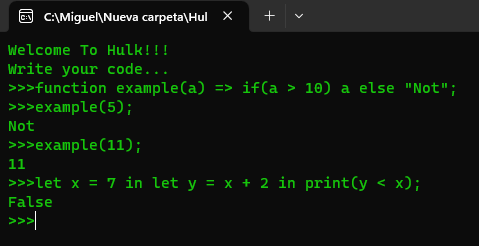
\includegraphics[width = 0.7\textwidth]{Example.png}
\caption{Ejemplo de C\'odigo en Hulk}
\end{figure}
~
\begin{center}
\textbf{Etapas del Proceso de Compilaci\'on}
\end{center}
\section{An\'alisis L\'exico(Tokenizaci\'on)}
Un \textbf{Token} no es m\'as que una seceuncia de car\'acteres, los cuales forman una cadena, que juntos cumplen ciertas caracter\'isticas ya predefinidas. Existen varios tipos de \textbf{Tokens}, como son: las palabras claves de alg\'un lenguaje (int, string, for, if), los nombres de las variables o las funciones (a, x, fib), los Operadores aritm\'eticos, de relaci\'on y l\'ogicos ($+$,$>=$,\&) y finalmente los literales num'ericos, cadenas o booleanos. 

La aplicaci'on utilza la clase Token, la cual define al objeto Token. En su campo se encuentra un enum \textbf{TokenType} almacenando todos los tipos de Tokens que utiliza el programa (La utilizaci\'on del enum se debe a que si se definen los tipos de Token mediante strings, es m\'as probable equivocarse al escribir un tipo de Token en alguna ocasi\'on).Adem\'as emplea un diccionario para guardar todos aquellos \textbf{Tokens} que est\'an prefijados en el lenguaje. El constructor de esta clase recibe un objeto de tipo \textbf{TokenType} y un string que representa el valor del Token. 

La clase est\'atica \textbf{Tokenizer} posee el m\'etodo GetTokens, el cual recibe la l\'inea de c\'odigo introducida por el usuario y realiza todo el proceso de Tokenizaci\'on de la misma, preguntando a cada car\'acter si es inicio, continuaci\'on o fin de Token. Una vez le\'ida y analizada la entrada, el m\'etodo devuelve la lista de Tokens correspondiente.

\section{An\'alisis Sint\'actico (Parser)}
En esta etapa, el Compilador obtiene la lista de Tokens previamente creada y procede a determinar si dicha lista (secuencia), es correcta. La definici\'on de una secuencia de Tokens correcta puede varirar en dependencia del lenguaje, en caso de HULK algunas secuencias incorrectas ser\'ian: una expresi\'on binaria que solo tenga un miembro, una expresi\'on no balanceada en cuanto a par\'entisis se refiere y otros casos. Para ello emplea una gram\'atica libre de contexto, en la cual est\'a reflejada la sintaxis de HULK. La gram\'atica empleada es la siguiente:\\

\begin{figure}[!h] \label{Gramatica}
\centering
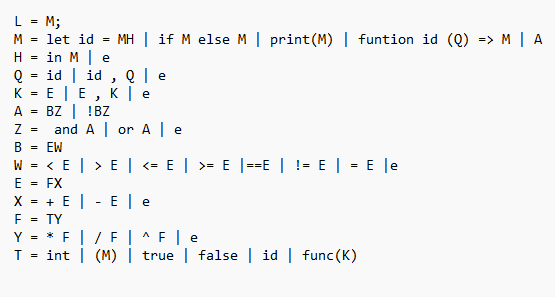
\includegraphics[width = 0.7\textwidth]{Gramatica.png}
\caption{Gram\'atica}
\end{figure}

Esta etapa no solo analiza si la secuencia de Tokens cumplen con la Sintaxis de HULK, adem\'as genera el \'Arbol de Sintaxis Abstracta (AST seg\'un sus siglas en Ingl\'es). En este AST, los nodos son las operaciones que se llevaran a cabo y los hijos son los operandos, estos a su vez pueden estar compuestos por otras operaciones. Con el AST se logra definir la instrucci\'on que se le dar\'a al Compilador de una manera recursiva.\\ 

Para lograr generar el AST, se emplea la clase abastracta \textbf{Expression}. Al utilizarse el modificador \textbf{abstract} se tiene la ventaja de que si se crea un nuevo objeto que herede de Expression, este podr\'a implementar todos sus m\'etodos de forma independiente, en dependencia del tipo de expresi\'on y de las necesidades del nuevo objeto.\\

\section{An\'alisis Sem\'antico}
Una vez creado el AST, durante el an\'alisi sem\'antico se desea saber si todos las operaciones est\'an trbajando con los operandos correctos, por ejemplo si la expresi\'on de suma, est\'a trabajando con dos n\'umeros o con dos expresiones que devuelvan un n\'umero o con dos varibles que tienen como valor un n\'umero. Es un trabajo bastante complejo, pero gracias a la definici\'on recursiva de la expresi\'on (AST) se puede realizar de una forma no muy complicada.\\

Teniendo en cuenta que se est\'a trabajando con la estructura de datos conocida como \'Arbol, la forma m\'as c\'omoda de operar con dicha estructura es recorri\'endolo. El recorrido que se emplea en esta casi\'on es en pre-orden, es decir, partiendo desde la Ra\'iz. El an\'alisis Sem\'antico realiza dos recorridos: 
\begin{itemize}
\item El primero para crear el \textbf{Scope} de la expres\'on, asi como los \textbf{Scopes} de las expresiones hijas, en caso de ser necesario.  
\item El segundo para verficar si las operaciones est\'an utilizando el tipo de operando correspondiente
\end{itemize}

La creaci\'on de los Scopes se basa en determinar en que \'ambito fue declarado una variable y en cual ser\'a usado. La definici\'on de Scope para esta aplicaci\'on, consiste en una estructura enlazable muy similar a la LinkedList (Estructura del lenguaje C\#), en la cual, cada Scope tiene acceso al Scope, valga la redondancia, que est\'a en el nivel inmediato superior. De esta forma, si se quiere saber que valor posee una variable, basta con recorrer los Scopes de los niveles superiores en donde esta se est\'a usando. \\

El chequeo de tipos, es el pen\'ultimo paso que se realiza antes de proceder con la evaluaci\'on de la expresi\'on. El Scope de la expresi\'on ya est\'a creado y tiene almacenados todos las variables declaradas y los tipos de datos que almacenan dichas variables. Evidentemente, la soluci\'on al problema de chequear si una expres\'on de suma opera con dos n\'umeros es, como bien se mencion\'o anteriormente, recorrer el AST una vez m\'as. Durante el recorrido cada vez que se se analice una operaci\'on, se pedir\'a el tipo de datos que representan los hijos de dicha expres\'on, si son los correctos, el recorrido continuar\'a.\\

\section{Evaluac\'on}
Una vez analizada l\'exica, sint\'actica y sem\'anticamente la entrada del usuario, se procede con la evaluaci\'on de la misma y se devuelve el resultado correspondiente.

\begin{center}
\textbf{Otros Detalles}
\end{center}

\section*{Sobre los Errores}
Existen tres tipos de errores, en el lenguaje HULK, estos ser\'ian: Error L\'exico, Error Sint\'actico y Error Sem\'antico. Evidentemente el nombre de cada error, da pista con respecto a en que momento del proceso podr\'ian ser lanzados.
\begin{itemize}
\item Error L\'exico: Como bien indica su nombre, aparece durante la etapa de an\'alisi l\'exico y normalmente se debe a expresiones que contengan tokens inv\'alidos (14a, "Hola).
\item Error Sint\'actico: Durante el proceso de Parser, como se mencion\'o anteriormente, se revisa si una secuencia de tokens es v\'alida o no, en caso de no serlo a parece este error. Algunos ejemplos de cadenas inv\'alidas ser\'ian: if(+ 5), $(8 - 5) * 3)$, @ "example".
\item Error Sem\'antico: Este error puede encontrarse en dos ocasiones. La primera ser\'ia durante la creaci\'on del Scope, en donde se revisa si se utiliza una varible previamente creada o se llama alguna funci\'on almacenada en la memoria. La segunda ocasi\'on es durante el chequeo el tipos, donde se determina si las operaciones est\'an usando los operandos correspondientes, un ejemplo de una sentencia inv\'alida ser\'ia: 80 + "Azul" \'o "Rojo" * true.\\
\end{itemize}

\section*{Sobre la clase Expression}
La clase abstracta Expression, es la clase fundamental de la alicaci\'on. El m\'etodo GetScope, es quien recorre el AST (quien en este caso es la expresi\'on devuelta por el Parser) y crea los scopes correspondientes, n\'otese que cada tipo que herede de Expression, rellenar\'a el Scope actual que es pasado como par\'ametro. El m\'etodo SemanticWalk, procede con el chequeo de tipos una vez creado el Scope en el m\'etodo antes mencionado. Finalmente Evaluate realiza la acci\'on de evaluar la entrada del usuario y devolver el resultado. Recalcar que al ser Expression una clase abastracta todos los tipos que hereden de esta, tendr\'an su propia implementaci\'on de estos m\'etodos.\\
 \begin{figure}[!h] \label{Expression}
 \centering
 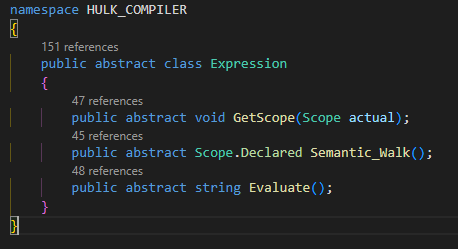
\includegraphics[width = 0.7\textwidth]{Expression.png}
 \caption{Expression}
 \end{figure}
 
 \begin{center}
 \textbf{Conclusiones}
 \end{center}
La aplicaci\'on presentada, se considera un compilador de una versi\'on mimnimalista del lenguaje HULK. Sin embargo est\'a capacitada para leer y realizar operaciones con instrucciones que posean cualquier tipo de operaci\'on aritm\'etica, condicionales, declaraci\'on de funciones, llamado de funciones e incluso la capacidad de evaluar funciones con implementaci\'on recursiva.
\begin{center}
\textbf{Bibligraf\'ia Consultada}
\begin{enumerate}
\item Compylers by Piad: Libro utilizado para el estudio de la asignatura Compilaci\'on. Autor: DrC. Alejandro Piad Morffis, profesor de la Facultad de Matem\'atica y Computaci\'on de la Universidad de La Habana.
\item Art\'iculos de Wikipedia en idioma ingl\'es que abordan temas de An\'alisis L\'exico, Sint\'actico y Sem\'antico
\end{enumerate}
\end{center}
\end{document}